\documentclass[border=0pt]{standalone}
% Match the Computer Modern text and mathematics of main.tex and its circuits.
\usepackage{fix-cm}
\usepackage{amsmath,amssymb,graphicx,xcolor,tikz,quantikz}
\usetikzlibrary{arrows.meta,calc}
\definecolor{PCS}{HTML}{17658B}
\definecolor{QCS}{HTML}{884366}
\definecolor{Ink}{HTML}{20242A}
\newcommand{\panel}[3]{\node[anchor=north west,font=\bfseries\fontsize{8}{9}\selectfont] at (#1,#2) {#3};}
\tikzset{every node/.style={font=\fontsize{7}{8}\selectfont,text=Ink,inner sep=0pt},
 flow/.style={-{Stealth[length=1.4mm,width=.9mm]},line width=.45pt},
 frame/.style={draw=black!50,line width=.25pt},
 operator/.append style={fill=white,draw=Ink,line width=.4pt}}
\DeclareMathSizes{6}{6}{5}{5}
\DeclareMathSizes{6.5}{6.5}{5}{5}
\DeclareMathSizes{7}{7}{5}{5}
\DeclareMathSizes{8}{8}{6}{5}
\pagestyle{empty}

% One physical gate size in both Figure 1 overview circuits.
\newcommand{\squaregate}[3]{%
 \draw[draw=Ink,fill=white,line width=.4pt] (#1-3,#2-3) rectangle (#1+3,#2+3);
 \node[font=\fontsize{8}{9.5}\selectfont] at (#1,#2) {$#3$};}
\tikzset{state label/.style={anchor=base,font=\fontsize{8}{9.5}\selectfont},
 operation label/.style={anchor=base,font=\fontsize{8}{9.5}\selectfont},
 group rule/.style={draw=black!35,line width=.3pt}}

% Coordinate annotations are lighter and smaller than operator arrows.
\tikzset{coordinate guide/.style={-{Stealth[length=.8mm,width=.55mm]},draw=black!60,line width=.3pt},
 coordinate label/.style={font=\fontsize{8}{9.5}\selectfont,text=black!70}}

\begin{document}
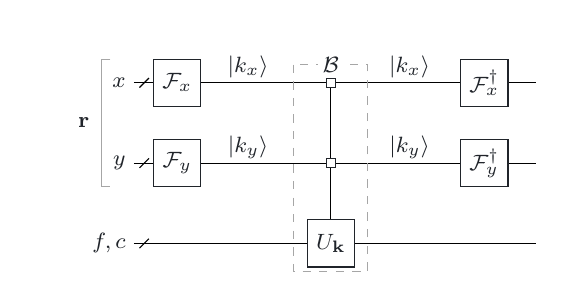
\begin{tikzpicture}[x=1mm,y=-1mm]
\path[use as bounding box] (0,0) rectangle (65,31.5);
% Two address registers form the joint pixel address; features are separate.
\draw[group rule] (10.5,4)--(9.4,4)--(9.4,20.2)--(10.5,20.2);
\node[anchor=east,font=\fontsize{8}{9.5}\selectfont] at (7.9,12.1) {$\mathbf r$};
\foreach \yy/\reg in {7/x,17.2/y,27.4/{f,c}}{
 \node[anchor=east,font=\fontsize{8}{9.5}\selectfont] at (12.5,\yy) {$\reg$};
 \draw[line width=.4pt] (13.5,\yy)--(64.5,\yy);
 \draw[line width=.4pt] (14.2,\yy+.6)--(15.4,\yy-.6);
}
\foreach \yy/\axis in {7/x,17.2/y}{
 \squaregate{19}{\yy}{\mathcal F_\axis}
 \squaregate{58}{\yy}{\mathcal F_\axis^{\dagger}}
 \node[anchor=base,font=\fontsize{8}{9.5}\selectfont] at (28,\yy-1.3) {$\ket{k_\axis}$};
 \node[anchor=base,font=\fontsize{8}{9.5}\selectfont] at (48.5,\yy-1.3) {$\ket{k_\axis}$};
}
% Both preserved Fourier indices jointly select a single feature unitary.
\draw[line width=.4pt] (38.5,7)--(38.5,27.4);
\foreach \yy in {7,17.2}{
 \draw[draw=Ink,fill=white,line width=.4pt] (37.9,\yy-.6) rectangle (39.1,\yy+.6);
}
\squaregate{38.5}{27.4}{U_{\mathbf k}}
\draw[draw=black!35,line width=.3pt,dashed] (33.8,4.7) rectangle (43.2,31);
\node[fill=white,inner xsep=.65mm,inner ysep=.15mm,font=\fontsize{8}{9.5}\selectfont] at (38.5,4.7) {$\mathcal B$};
\end{tikzpicture}
\end{document}
